\documentclass[12pt,a4paper]{article}
\usepackage[utf8]{inputenc}
\usepackage[T1]{fontenc}
\usepackage[spanish]{babel}
\usepackage[margin=2.2cm]{geometry}
\usepackage{xcolor}
\usepackage[most]{tcolorbox}
\usepackage{enumitem}
\usepackage{array}
\usepackage{longtable}
\usepackage{fancyhdr}
\usepackage{lmodern}
\usepackage{graphicx}

% ===== CAMBIA AQUÍ TUS DATOS =====
\newcommand{\minombre}{[Tu nombre y apellido]}
\newcommand{\micurso}{6° básico}
% ================================

\definecolor{magenta}{HTML}{C8227A}
\definecolor{verde}{HTML}{1F8A4C}
\definecolor{oro}{HTML}{E0A614}
\definecolor{tinta}{HTML}{2D1F3D}

\setlength{\headheight}{15pt}
\pagestyle{fancy}
\fancyhf{}
\lhead{\small Guion · El caballero de la armadura oxidada}
\rhead{\small \minombre}
\cfoot{\small \thepage}
\setlength{\parindent}{0pt}
\setlength{\parskip}{6pt}

% Lo que se dice en voz alta
\newtcolorbox{digo}{enhanced, breakable, colback=white, colframe=verde,
  boxrule=1pt, arc=3mm, left=8pt, right=8pt, top=6pt, bottom=6pt,
  title={\textbf{Lo que digo}}, fonttitle=\small\bfseries, coltitle=white}

% Número del paso (círculo magenta)
\newcommand{\num}[1]{\tikz[baseline=(c.base)]\node[circle, fill=magenta, text=white,
  font=\bfseries\small, inner sep=1.5pt, minimum size=1.45em](c){#1};}

% Paso: imagen de la cartulina con el número + título, tiempo y qué señalar
\newcommand{\paso}[4]{%
  \vspace{10pt}
  \begin{tcolorbox}[enhanced, sidebyside, sidebyside align=top seam, lefthand width=2.7cm,
    colback=magenta!5, colframe=magenta, boxrule=1pt, arc=2mm,
    left=5pt, right=8pt, top=5pt, bottom=5pt, segmentation hidden]
    \includegraphics[width=\linewidth]{imagenes_guion/paso#1.jpg}
    \tcblower
    {\Large\num{#1}}\ {\large\bfseries\color{magenta} #2}\hfill\textbf{#3}\par\medskip
    \textcolor{magenta}{\textbf{SEÑALO EN LA CARTULINA:}} #4
  \end{tcolorbox}\vspace{-4pt}}

% Consejo de cómo decirlo (lenguaje no verbal / voz)
\newcommand{\como}[1]{%
  \begin{tcolorbox}[colback=oro!12, colframe=oro, boxrule=0.6pt, arc=2mm,
    left=6pt, right=6pt, top=3pt, bottom=3pt]
    \textbf{Cómo lo digo:} #1
  \end{tcolorbox}}

\begin{document}

\begin{center}
  {\LARGE\bfseries\color{magenta} Guion de mi disertación}\\[4pt]
  {\Large\bfseries El caballero de la armadura oxidada}\\[2pt]
  {\large Robert Fisher}\\[8pt]
  \minombre\ \,·\, \micurso\ \,·\, Duración: \textbf{9 minutos aprox.} (máximo 10)
\end{center}

\section*{Antes de empezar}
\begin{itemize}[leftmargin=*,itemsep=2pt]
  \item Llegar a la hora, con el \textbf{uniforme completo y ordenado}, la cartulina y el computador o pendrive listos.
  \item Abrir el archivo \texttt{index.html}. Apretar \textbf{F} para pantalla completa y \textbf{T} para ver el cronómetro. Con la flecha \textbf{$\rightarrow$} avanzo y con \textbf{$\leftarrow$} retrocedo.
  \item Pararme \textbf{al lado de la cartulina}, mirando al curso. Nunca de espalda.
  \item Hablar \textbf{fuerte, lento y claro}. Mirar a distintos compañeros, no solo a la profesora.
  \item Este guion es para \textbf{estudiarlo}, no para leerlo. Lo puedo tener en la mano solo por si me pierdo.
  \item Si algo falla (el computador no prende), \textbf{mantengo la calma}: uso solo la cartulina, porque el guion dice qué señalar.
\end{itemize}

\section*{Mapa de la cartulina}
Cada número es un \textbf{paso}: indica el orden en que voy señalando la cartulina. Es el mismo número de la
diapositiva que se ve en el computador.

\begin{center}
  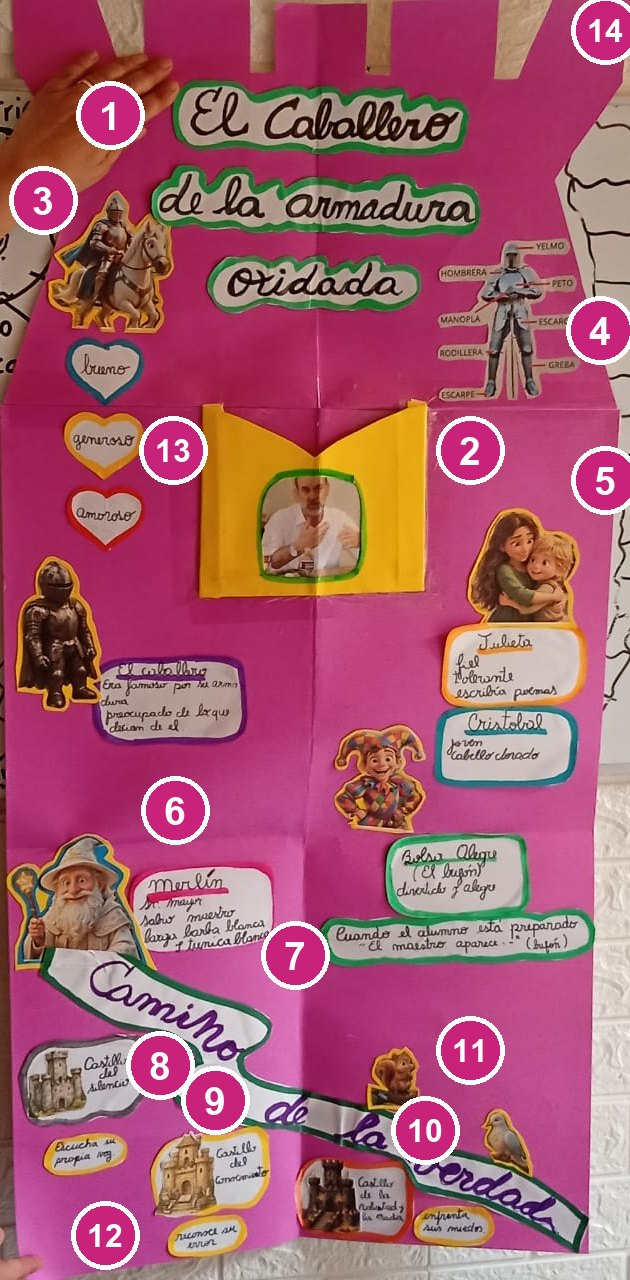
\includegraphics[height=12cm]{imagenes_guion/mapa.jpg}
\end{center}

\section*{Tabla de tiempos}
\begin{center}
\begin{tabular}{>{\centering}p{1.3cm} p{7.8cm} >{\centering\arraybackslash}p{2.2cm}}
\textbf{Paso} & \textbf{Parte} & \textbf{Tiempo} \\ \hline
1--2 & Introducción: saludo, libro, autor y de qué trata & 1:15 \\
3--6 & Personajes (físico y psicológico) & 3:00 \\
7--11 & El problema y el Camino de la Verdad & 2:45 \\
12--13 & Mi opinión y mi solución & 1:30 \\
14 & Cierre y preguntas & 0:30 \\ \hline
 & \textbf{Total} & \textbf{9:00} \\
\end{tabular}
\end{center}

\newpage
% ================================================================
\section*{\color{verde}INTRODUCCIÓN}

\paso{1}{Portada}{0:30}{el \textbf{título} arriba de la cartulina, pasando la mano por las tres líneas.}
\begin{digo}
Buenos días, profesora y compañeros. Mi nombre es \minombre\ y hoy les voy a presentar el libro
\textbf{\emph{El caballero de la armadura oxidada}}, escrito por \textbf{Robert Fisher}.
\end{digo}
\como{sonreír, mirar al curso, pararse derecha y esperar que todos estén en silencio antes de hablar.}

\paso{2}{¿De qué trata?}{0:45}{la \textbf{foto del autor} en el libro amarillo, al centro.}
\begin{digo}
Él es Robert Fisher, el autor del libro.\\[4pt]
Este libro cuenta la historia de un caballero que quería ser el mejor de todo el reino. Usaba tanto su armadura que un día
\textbf{quedó atrapado dentro de ella}. Para poder salir, tuvo que recorrer un camino muy especial: el \textbf{Camino de la Verdad}.\\[4pt]
Hoy les voy a contar cómo son los personajes, cuál es el problema, cómo es el camino, qué me pareció el libro y qué
solución le daría yo al caballero.
\end{digo}
\como{al decir “hoy les voy a contar”, contar con los dedos las cinco partes.}

% ================================================================
\section*{\color{verde}DESARROLLO}

\paso{3}{El Caballero}{1:00}{primero el \textbf{caballero a caballo}, después los \textbf{tres corazones} (uno por uno) y al final la \textbf{tarjeta del caballero} con la armadura oscura.}
\begin{digo}
El personaje principal es el caballero.\\[4pt]
\textbf{Por fuera}, tenía una armadura tan brillante que se veía desde lejos, y andaba a caballo luchando contra dragones
y rescatando doncellas.\\[4pt]
\textbf{Por dentro}, era una persona \textbf{buena}, \textbf{generosa} y \textbf{amorosa}. Pero también tenía un defecto: estaba
muy \textbf{preocupado de lo que decían de él}. Quería que todos lo admiraran.\\[4pt]
Por eso, nunca se sacaba la armadura. ¡La usaba hasta para comer y para dormir! Y pasó tanto tiempo así que su familia
\textbf{se olvidó de cómo era su cara}. Esto muestra que, aunque era bueno, se preocupaba más de su fama que de las personas que lo querían.
\end{digo}

\paso{4}{La armadura}{0:35}{la \textbf{armadura con sus partes}, arriba a la derecha. Ir tocando de arriba hacia abajo: yelmo, hombrera, peto, manopla, escarcela, rodillera, greba y escarpe.}
\begin{digo}
Aquí les muestro las partes de una armadura: el yelmo protege la cabeza, el peto el pecho y los escarpes los pies.\\[4pt]
En el libro, la armadura es muy importante, porque lo \textbf{protegía} en las batallas, pero también \textbf{escondía lo que sentía}.
Con la armadura nadie podía ver cómo era él de verdad.
\end{digo}

\paso{5}{Julieta y Cristóbal}{0:45}{la \textbf{mamá abrazando a su hijo} y las tarjetas de \textbf{Julieta} y \textbf{Cristóbal}, en el lado derecho.}
\begin{digo}
Su familia era Julieta y Cristóbal.\\[4pt]
\textbf{Julieta} era su esposa. Era \textbf{fiel}, porque siempre lo esperaba; \textbf{tolerante}, porque aguantó mucho tiempo
que él se fuera a las batallas; y le gustaba \textbf{escribir poemas}. Pero un día se cansó de no poder ver a su esposo y
le pidió que eligiera entre ella y la armadura.\\[4pt]
\textbf{Cristóbal} era su hijo, un niño de \textbf{cabello dorado}. Él casi no conocía la cara de su papá, y eso lo ponía triste.
\end{digo}
\como{cambiar la voz a una más suave al hablar de Julieta y Cristóbal.}

\paso{6}{Merlín y Bolsalegre}{0:45}{\textbf{Merlín} a la izquierda, después el \textbf{bufón} y la tarjeta de \textbf{Bolsalegre}, y al final la \textbf{frase} de abajo.}
\begin{digo}
Los personajes que lo ayudan son Merlín y Bolsalegre.\\[4pt]
\textbf{Merlín} es un mago. Es un \textbf{señor mayor}, con \textbf{larga barba blanca} y \textbf{túnica blanca}. Es un
\textbf{sabio maestro}: no le resuelve los problemas al caballero, sino que le enseña a resolverlos solo.\\[4pt]
\textbf{Bolsalegre} es el bufón. Es \textbf{divertido y alegre}, y le cuenta al caballero que Merlín puede ayudarlo.\\[4pt]
En la cartulina puse una frase muy importante del libro: \textbf{“Cuando el alumno está preparado, el maestro aparece”}.
Para mí significa que la ayuda llega cuando uno de verdad quiere cambiar.
\end{digo}
\como{decir la frase más lento y mirando al curso.}

\paso{7}{El problema}{0:30}{la cinta grande \textbf{“Camino de la verdad”}, pasando la mano por toda la cinta.}
\begin{digo}
El problema de la historia es que \textbf{la armadura se quedó pegada}. Se había \textbf{oxidado} y nadie se la pudo sacar,
ni siquiera el herrero. Su familia ya no podía verlo ni abrazarlo.\\[4pt]
Entonces el caballero va a buscar a Merlín al bosque, y Merlín le dice que para sacarse la armadura debe recorrer el
\textbf{Camino de la Verdad}. En ese camino hay tres castillos.
\end{digo}

\paso{8}{Castillo del Silencio}{0:40}{el \textbf{primer castillo}, abajo a la izquierda, y la nota \textbf{“Escucha su propia voz”}.}
\begin{digo}
El primer castillo es el \textbf{Castillo del Silencio}. Ahí no había nadie con quién hablar, y el caballero se dio cuenta de
que nunca había escuchado de verdad a los demás.\\[4pt]
En el silencio aprendió a \textbf{escuchar su propia voz}, es decir, lo que él sentía de verdad. Se puso a llorar, y con sus
lágrimas \textbf{una parte de la armadura se cayó}.
\end{digo}

\paso{9}{Castillo del Conocimiento}{0:40}{el \textbf{segundo castillo}, abajo al centro, y la nota \textbf{“Reconoce sus errores”}.}
\begin{digo}
El segundo es el \textbf{Castillo del Conocimiento}. Era muy oscuro, y solo se iluminaba cuando el caballero entendía algo nuevo.\\[4pt]
Aquí el caballero \textbf{reconoce sus errores}: se da cuenta de que le importaba más ser famoso que estar con su familia.
Al entender esto, \textbf{otra parte de la armadura se cayó}.
\end{digo}

\paso{10}{Castillo de la Voluntad y la Osadía}{0:40}{el \textbf{tercer castillo}, abajo a la derecha, y la nota \textbf{“Enfrenta sus miedos”}.}
\begin{digo}
El tercero es el \textbf{Castillo de la Voluntad y la Osadía}. Lo cuidaba el \textbf{Dragón del Miedo y la Duda}.\\[4pt]
Al principio el caballero quería escapar, pero decidió \textbf{enfrentar sus miedos}. Lo más interesante es que, mientras
más valiente era el caballero, \textbf{más pequeño se hacía el dragón}, hasta que desapareció.
\end{digo}
\como{hacer un gesto con las manos de algo que se achica al hablar del dragón.}

\paso{11}{La Cima de la Verdad}{0:35}{la \textbf{ardilla} y la \textbf{paloma} que están sobre la cinta del camino.}
\begin{digo}
Al final llega a la \textbf{Cima de la Verdad}. Para subir, tenía que \textbf{soltarse y confiar}. Cuando lo hizo, lloró de
alegría y \textbf{la armadura se cayó completa}. Por fin era libre.\\[4pt]
En todo el viaje lo acompañaron dos amigos: \textbf{la ardilla} y \textbf{la paloma Rebeca}, que lo ayudaron y no lo dejaron solo.
\end{digo}

% ================================================================
\section*{\color{verde}CIERRE}

\paso{12}{Mi opinión}{0:50}{pasar la mano por los \textbf{tres castillos}, de izquierda a derecha.}
\begin{digo}
Ahora les voy a contar qué me pareció el libro.\\[4pt]
Lo que \textbf{más me gustó} fueron los tres castillos, porque en cada uno el caballero aprende algo y se le cae un pedazo
de armadura. Por ejemplo, en el Castillo del Silencio, solo por escucharse a sí mismo, ya empezó a cambiar.\\[4pt]
Lo que \textbf{menos me gustó} fue el principio, cuando deja sola a su familia por ir a tantas batallas. Me dio pena
Cristóbal, porque no conocía la cara de su papá.\\[4pt]
Mi opinión es que es \textbf{un libro muy bueno}, porque enseña que ser valiente no es solo pelear con dragones:
también es \textbf{mostrar lo que uno siente} y reconocer cuando se equivoca.\\[4pt]
Esto me hizo pensar en mi propia vida: a veces yo también digo que estoy bien cuando estoy triste, y me siento mucho mejor cuando se lo cuento a alguien de confianza.
\end{digo}

\paso{13}{Mi solución}{0:40}{volver a los \textbf{tres corazones} y después a \textbf{Julieta con Cristóbal}.}
\begin{digo}
Si yo fuera el caballero, haría tres cosas para no quedar atrapado:\\[4pt]
\textbf{Primero}, me sacaría la armadura apenas llegara a mi casa. \textbf{Segundo}, escucharía a Julieta y jugaría con
Cristóbal. \textbf{Tercero}, pediría ayuda apenas me sintiera atrapado, sin esperar tanto.\\[4pt]
Creo que esta solución sirve porque el caballero \textbf{ya era bueno, generoso y amoroso}. No necesitaba ser famoso:
solo tenía que demostrar su cariño a su familia.
\end{digo}
\como{contar con los dedos: uno, dos, tres.}

\paso{14}{Para terminar}{0:30}{abrir los brazos y mostrar \textbf{toda la cartulina}.}
\begin{digo}
Para terminar, este libro me enseñó que todos podemos tener una “armadura”: por ejemplo, cuando hacemos como que estamos
bien pero estamos tristes, o cuando escondemos lo que sentimos.\\[4pt]
Los invito a \textbf{leer este libro}, porque es corto, entretenido y te hace pensar.\\[4pt]
\textbf{Muchas gracias por escucharme. ¿Alguien tiene alguna pregunta?}
\end{digo}
\como{esperar con calma. Escuchar la pregunta completa, decir “gracias por tu pregunta” y responder con mis palabras.}

\newpage
% ================================================================
\section*{Preguntas que me podrían hacer}

\textbf{1. ¿Por qué la armadura se oxidó?}\\
Porque el caballero la usó tanto tiempo, sin sacársela nunca, que se oxidó y se quedó pegada a su cuerpo.

\textbf{2. ¿Qué significa la armadura en el libro?}\\
Significa todo lo que usamos para escondernos y para que los demás no vean lo que sentimos de verdad.

\textbf{3. ¿Por qué se caía la armadura cuando lloraba?}\\
Porque cuando lloraba era sincero con lo que sentía. Al mostrar sus sentimientos ya no necesitaba la armadura.

\textbf{4. ¿Quién te gustó más, aparte del caballero?}\\
Merlín, porque es un buen maestro: no le daba las respuestas, lo ayudaba a encontrarlas solo.

\textbf{5. ¿Qué harías tú si fueras Julieta?}\\
Le diría lo que siento y le pediría que pasemos más tiempo juntos, igual que ella hizo en el libro.

\textbf{Si no sé la respuesta:} digo con calma “Buena pregunta, no lo recuerdo bien, pero creo que…” y respondo lo que pienso.

\vspace{8pt}
% ================================================================
\section*{Revisión con la rúbrica}
\renewcommand{\arraystretch}{1.25}
\begin{longtable}{p{5.4cm} p{10.2cm}}
\textbf{Criterio} & \textbf{Dónde lo cumplo} \\ \hline
\endhead
Presentación (saludo, nombre, libro, autor) & Paso 1: saludo, mi nombre, título completo y autor. \\
Estructura (introducción, desarrollo, cierre) & Paso 2 anuncia las partes; el pie de cada diapositiva marca Introducción, Desarrollo o Cierre. \\
Descripción física y psicológica (mín. 3) & Caballero, Julieta, Cristóbal y Merlín, con características unidas a lo que hacen (pasos 3 a 6). \\
Opinión fundamentada & Paso 12: “es un libro muy bueno porque…”. \\
Argumentación con ejemplos & Ejemplos del libro: la armadura para dormir, Cristóbal sin conocer la cara de su papá, el Castillo del Silencio. \\
Propuesta de solución al conflicto & Paso 13: tres acciones y por qué funcionarían. \\
Apreciación personal (más y menos) & Paso 12: lo que más y lo que menos me gustó, con ejemplos. \\
Gusto por la lectura & Paso 14: invito a leer el libro. \\
Pertinencia y dominio del tema & Todo lo que digo es del libro; me sé la historia en orden. \\
Uso de material de apoyo & En cada paso señalo una parte de la cartulina, en el orden del mapa. \\
Lenguaje verbal & Voz fuerte, lenta y clara; cambio el tono en las partes importantes. \\
Lenguaje no verbal & De frente al curso, con contacto visual y gestos (contar con los dedos, mostrar la cartulina). \\
Fluidez y autonomía & Estudio el guion; no leo las diapositivas ni las fichas. \\
Vocabulario y registro formal & Uso palabras como “psicológico”, “tolerante”, “osadía” y “reconocer”; nada de “o sea” ni “cachai”. \\
Comprensión (palabras propias) & Todo está con mis palabras; puedo explicar cada palabra difícil. \\
Manejo del tiempo & 9 minutos; uso el cronómetro (tecla T). Si falla algo, sigo con la cartulina. \\
Atención a preguntas & Tengo preparadas 5 respuestas (página anterior). \\
Presentación personal y puntualidad & Uniforme completo, llegar a la hora con todo listo. \\
Respeto a los compañeros & Escucho en silencio las disertaciones de los demás. \\
Ortografía del material & Revisar que la cartulina y las diapositivas no tengan errores. \\
\end{longtable}

\section*{Palabras que debo saber explicar}
\begin{itemize}[leftmargin=*,itemsep=1pt]
  \item \textbf{Oxidada:} cuando el metal se pone café y se echa a perder por el agua y el aire.
  \item \textbf{Tolerante:} que acepta y tiene paciencia con los demás.
  \item \textbf{Osadía:} valentía para atreverse a hacer algo difícil.
  \item \textbf{Psicológico:} cómo es una persona por dentro: lo que piensa y siente.
  \item \textbf{Bufón:} persona que hacía reír al rey y a la gente del castillo.
\end{itemize}

\newpage
% ================================================================
\section*{\color{verde}Guion completo (para estudiar de corrido)}
{\small Cada número en círculo es el paso del mapa: ahí señalo esa parte de la cartulina y avanzo la diapositiva.}

\begin{center}
  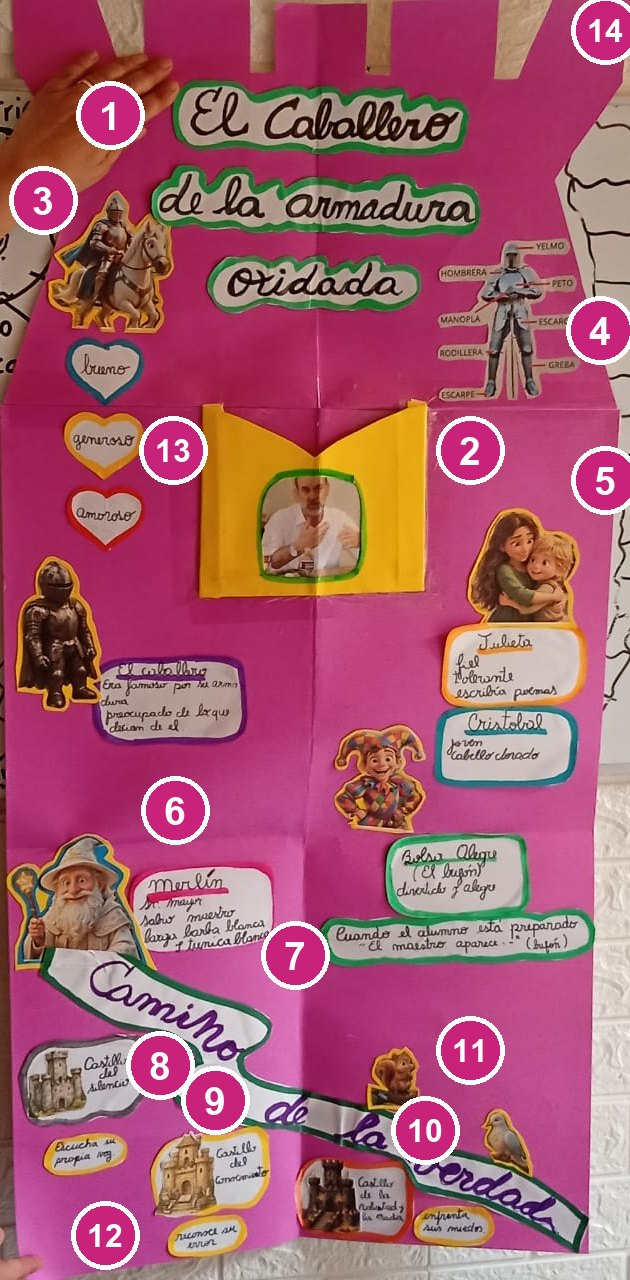
\includegraphics[height=9cm]{imagenes_guion/mapa.jpg}
\end{center}

\begin{tcolorbox}[enhanced, breakable, colback=verde!6, colframe=verde, boxrule=1.2pt,
  arc=3mm, left=10pt, right=10pt, top=8pt, bottom=8pt, coltext=verde!70!black]
\setlength{\parskip}{7pt}
\newcommand{\cambio}[1]{\num{#1}\ }

\cambio{1}Buenos días, profesora y compañeros. Mi nombre es \minombre\ y hoy les voy a presentar el libro
\emph{El caballero de la armadura oxidada}, escrito por Robert Fisher.

\cambio{2}Él es Robert Fisher, el autor del libro. Este libro cuenta la historia de un caballero que quería ser
el mejor de todo el reino. Usaba tanto su armadura que un día quedó atrapado dentro de ella. Para poder salir, tuvo que
recorrer un camino muy especial: el Camino de la Verdad. Hoy les voy a contar cómo son los personajes, cuál es el problema,
cómo es el camino, qué me pareció el libro y qué solución le daría yo al caballero.

\cambio{3}El personaje principal es el caballero. Por fuera, tenía una armadura tan brillante que se veía desde
lejos, y andaba a caballo luchando contra dragones y rescatando doncellas. Por dentro, era una persona buena, generosa y
amorosa. Pero también tenía un defecto: estaba muy preocupado de lo que decían de él. Quería que todos lo admiraran. Por
eso, nunca se sacaba la armadura. ¡La usaba hasta para comer y para dormir! Y pasó tanto tiempo así que su familia se
olvidó de cómo era su cara. Esto muestra que, aunque era bueno, se preocupaba más de su fama que de las personas que lo querían.

\cambio{4}Aquí les muestro las partes de una armadura: el yelmo protege la cabeza, el peto el pecho y los
escarpes los pies. En el libro, la armadura es muy importante, porque lo protegía en las batallas, pero también escondía
lo que sentía. Con la armadura nadie podía ver cómo era él de verdad.

\cambio{5}Su familia era Julieta y Cristóbal. Julieta era su esposa. Era fiel, porque siempre lo esperaba;
tolerante, porque aguantó mucho tiempo que él se fuera a las batallas; y le gustaba escribir poemas. Pero un día se cansó
de no poder ver a su esposo y le pidió que eligiera entre ella y la armadura. Cristóbal era su hijo, un niño de cabello
dorado. Él casi no conocía la cara de su papá, y eso lo ponía triste.

\cambio{6}Los personajes que lo ayudan son Merlín y Bolsalegre. Merlín es un mago. Es un señor mayor, con
larga barba blanca y túnica blanca. Es un sabio maestro: no le resuelve los problemas al caballero, sino que le enseña a
resolverlos solo. Bolsalegre es el bufón. Es divertido y alegre, y le cuenta al caballero que Merlín puede ayudarlo. En la
cartulina puse una frase muy importante del libro: “Cuando el alumno está preparado, el maestro aparece”. Para mí significa
que la ayuda llega cuando uno de verdad quiere cambiar.

\cambio{7}El problema de la historia es que la armadura se quedó pegada. Se había oxidado y nadie se la pudo
sacar, ni siquiera el herrero. Su familia ya no podía verlo ni abrazarlo. Entonces el caballero va a buscar a Merlín al
bosque, y Merlín le dice que para sacarse la armadura debe recorrer el Camino de la Verdad. En ese camino hay tres castillos.

\cambio{8}El primer castillo es el Castillo del Silencio. Ahí no había nadie con quién hablar, y el caballero
se dio cuenta de que nunca había escuchado de verdad a los demás. En el silencio aprendió a escuchar su propia voz, es decir,
lo que él sentía de verdad. Se puso a llorar, y con sus lágrimas una parte de la armadura se cayó.

\cambio{9}El segundo es el Castillo del Conocimiento. Era muy oscuro, y solo se iluminaba cuando el caballero
entendía algo nuevo. Aquí el caballero reconoce sus errores: se da cuenta de que le importaba más ser famoso que estar con
su familia. Al entender esto, otra parte de la armadura se cayó.

\cambio{10}El tercero es el Castillo de la Voluntad y la Osadía. Lo cuidaba el Dragón del Miedo y la Duda. Al
principio el caballero quería escapar, pero decidió enfrentar sus miedos. Lo más interesante es que, mientras más valiente
era el caballero, más pequeño se hacía el dragón, hasta que desapareció.

\cambio{11}Al final llega a la Cima de la Verdad. Para subir, tenía que soltarse y confiar. Cuando lo hizo,
lloró de alegría y la armadura se cayó completa. Por fin era libre. En todo el viaje lo acompañaron dos amigos: la ardilla
y la paloma Rebeca, que lo ayudaron y no lo dejaron solo.

\cambio{12}Ahora les voy a contar qué me pareció el libro. Lo que más me gustó fueron los tres castillos,
porque en cada uno el caballero aprende algo y se le cae un pedazo de armadura. Por ejemplo, en el Castillo del Silencio,
solo por escucharse a sí mismo, ya empezó a cambiar. Lo que menos me gustó fue el principio, cuando deja sola a su familia
por ir a tantas batallas. Me dio pena Cristóbal, porque no conocía la cara de su papá. Mi opinión es que es un libro muy
bueno, porque enseña que ser valiente no es solo pelear con dragones: también es mostrar lo que uno siente y reconocer
cuando se equivoca. Esto me hizo pensar en mi propia vida: a veces yo también digo que estoy bien cuando estoy triste, y me siento mucho mejor cuando se lo cuento a alguien de confianza.

\cambio{13}Si yo fuera el caballero, haría tres cosas para no quedar atrapado. Primero, me sacaría la armadura
apenas llegara a mi casa. Segundo, escucharía a Julieta y jugaría con Cristóbal. Tercero, pediría ayuda apenas me sintiera
atrapado, sin esperar tanto. Creo que esta solución sirve porque el caballero ya era bueno, generoso y amoroso. No
necesitaba ser famoso: solo tenía que demostrar su cariño a su familia.

\cambio{14}Para terminar, este libro me enseñó que todos podemos tener una “armadura”: por ejemplo, cuando
hacemos como que estamos bien pero estamos tristes, o cuando escondemos lo que sentimos. Los invito a leer este libro,
porque es corto, entretenido y te hace pensar. Muchas gracias por escucharme. ¿Alguien tiene alguna pregunta?
\end{tcolorbox}

\newpage
% ================================================================
\section*{\color{verde}Observaciones: ¿cumple con la rúbrica?}
Revisión del guion y del material, criterio por criterio.
\textcolor{verde}{\textbf{CUMPLE}}: el guion ya lo resuelve.
\textcolor{oro!80!black}{\textbf{DEPENDE DE TI}}: el guion ayuda, pero se nota el día de la disertación.
\textcolor{magenta}{\textbf{A CORREGIR}}: hay que arreglarlo antes de presentar.

\newcommand{\si}{\textcolor{verde}{\textbf{CUMPLE}}}
\newcommand{\ojo}{\textcolor{oro!80!black}{\textbf{DEPENDE DE TI}}}
\newcommand{\no}{\textcolor{magenta}{\textbf{A CORREGIR}}}

\renewcommand{\arraystretch}{1.3}
\begin{longtable}{p{4cm} >{\raggedright\arraybackslash}p{3.1cm} p{8.5cm}}
\textbf{Criterio} & \textbf{Estado} & \textbf{Observación} \\ \hline
\endhead
\multicolumn{3}{l}{\textbf{\color{magenta}Ponderación 80\%}} \\
Descripción física y psicológica & \si & Más de 3 características del caballero (brillante armadura, bueno, generoso, amoroso, preocupado de lo que decían de él), unidas a lo que hace: usar la armadura hasta para dormir. También se describe a Julieta, Cristóbal, Merlín y Bolsalegre. \\
Opinión fundamentada & \si & Opina que es un libro muy bueno y explica por qué, usando el texto y una experiencia propia (paso 12). Si tienes un ejemplo de tu vida más real, cámbialo por el tuyo: así suena más natural. \\
Argumentación con ejemplos & \si & Da su postura frente al caballero (“se preocupaba más de su fama que de su familia”) con ejemplos concretos: la armadura para dormir y Cristóbal sin conocer la cara de su papá. \\
Propuesta de solución & \si & Tres acciones claras y por qué funcionarían (paso 13). \\
Apreciación personal & \si & Dice lo que más y lo que menos le gustó, y cada parte tiene un ejemplo del libro (paso 12). \\
Lenguaje no verbal & \ojo & El guion marca dónde señalar y qué gestos hacer. Falta practicar: mirar al curso, no dar la espalda a la cartulina y moverse un poco. \\
Lenguaje verbal & \ojo & Hablar fuerte, lento y cambiar el tono en las partes importantes. Conviene ensayar en voz alta frente a la familia. \\
Uso de material de apoyo & \si & La cartulina se usa en los 14 pasos y la presentación muestra cada parte. \\
Fluidez y autonomía & \ojo & Es el criterio con más riesgo: el guion tiene cerca de 1.000 palabras. Hay que estudiarlo hasta contarlo con tus palabras; no se lee. Usa el mapa numerado como ayuda. \\
Vocabulario y registro & \si & Registro formal y palabras variadas. Se cambió “o sea” por “es decir” para evitar muletillas. \\
Estructura & \si & Introducción (pasos 1--2), desarrollo (3--11) y cierre (12--14), con frases de paso: “Ahora les voy a contar…”, “Para terminar…”. \\
Pertinencia & \si & Todo lo que se dice es del libro. Las partes de la armadura se relacionan con lo que significa en la historia. \\
Dominio del tema & \ojo & El guion está hecho con la cartulina y la historia del libro, pero el texto del PDF no se pudo leer. Revisa con el libro estos detalles: el herrero, la ardilla y la paloma Rebeca, y quién dice la frase del maestro. \\[4pt]
\multicolumn{3}{l}{\textbf{\color{magenta}Ponderación 20\%}} \\
Presentación & \si & Saluda y dice el título exacto y el autor. Cambia \texttt{\textbackslash minombre} por tu \textbf{nombre completo}: la rúbrica lo pide así. \\
Presentación personal & \ojo & Uniforme completo y ordenado ese día. \\
Respeto hacia los compañeros & \ojo & Escuchar en silencio las disertaciones de los demás. \\
Ortografía en el material & \no & En la cartulina dice \textbf{“Cristobal”} y debe ser \textbf{“Cristóbal”} (con tilde). También dice \textbf{“Bolsa Alegre”} y en el libro es \textbf{“Bolsalegre”}. Revisa además las tildes de: escribía, túnica, Merlín, bufón y osadía. Con 1 a 3 errores el puntaje baja a Satisfactorio. Las diapositivas ya están revisadas. \\
Manejo del tiempo & \si & El guion dura cerca de 9 minutos y la presentación tiene cronómetro (tecla T). Si falla el computador, se puede seguir solo con la cartulina y el mapa. \\
Atención a preguntas & \si & Hay 5 preguntas preparadas y una frase para cuando no sepas la respuesta. \\
Responsabilidad y puntualidad & \ojo & Llegar a la hora con la cartulina, el pendrive y el guion impreso. \\
Comprensión (palabras propias) & \si & Todo está escrito como habla un estudiante de sexto, y las palabras difíciles están explicadas. \\
\end{longtable}

\begin{tcolorbox}[colback=magenta!6, colframe=magenta, arc=2mm]
\textbf{Antes de presentar:} (1) corregir “Cristóbal” y “Bolsalegre” en la cartulina, (2) poner tu nombre completo,
(3) ensayar al menos 3 veces con cronómetro, señalando la cartulina en el orden del mapa.
\end{tcolorbox}

\end{document}
